\section{Algorithm}


The core of the Naive Cartographer is a Markov decision process model pair:

A transition probability estimate and
\begin{equation}
p(s^\prime | s, a)
\end{equation}

A reward estimate
\begin{equation}
Q(s, a)
\end{equation}

(following the notation of Sutton and Barto). If you already have a mental model
of these, that will serve you well, but FNC puts its own spin on them.
These quirks, the deviations from the default vanilla interpretations,
are what makes FNC unique.

\subsection*{Quirk 1: Fuzzy state varibles}
\label{algofuzzy}

As mentioned above, FNC requires
all state values to be between 0 and 1 and interprets them as fuzzy variables.
The later implications of this are many, but they don't otherwise
look odd as a state representation. I'm not aware of any other RL modeling
approaches that take this approach.

\subsection*{Quirk 2: Conditional independence of features}
\label{algobayes}

The weirdest thing FNC does is assume that all of its features have
independent effects on the outcome of the model. This assumption
is patently wrong, but it is so helpful in taming the curse of
dimensionality that FNC gets good mileage out of it despite that.
This trade-off has been successful in natural language processing (NLP)
classification tasks under the name of Naive Bayes. As far as I know it's
never been applied to reinforcement learning.

This Naive assumption allows several tricks and shortcuts that will be
described in later paragraphs.

\subsection*{Quirk 3: Features instead of states}
\label{introstate}

This quirk is worth a closer look because it breaks some of
our hard won intuitions about state spaces.
Traditionally Markov Decision Processes (MDPs), describe an agent that
was in a state, $s$, took an action, $a$, and ended up in a new state,
$s^\prime$. 
FNC's state representation
is not actually a state representation at all. 
In physics, the state of an object is a specific set of information that
lets you know exactly what it's doing. In the case of a bowling ball,
if you know where it is, how fast it's moving, and how fast it's spinning,
you can predict everything it's going to do next with high accuracy.
The bowling ball's state consists of position, orientation, velocity,
and angular velocity, all in three dimensions. A physics simulator would
need all of these to represent the bowling ball. The notion of state in
MDPs is this holistic representation, and a good portion of RL analysis
subtly bakes in this assumption. 

FNC does not presuppose that all the state information is contained
in its inputs. MDP learning problems where what is observed is different
than the state of the system can be described as a
\href{https://en.wikipedia.org/wiki/Partially_observable_Markov_decision_process}{Partially observable Markov decision process}
(POMDP). POMDPs posit that there is a concise set of state variables,
but assumes that the sensors in use only reflect them indirectly.
This would be akin to estimating the state of the bowling ball based
only on the audio input from an array of microphones placed along the lane.
Unlike POMDPs, FNC takes the additional shortcut of ignoring the
underlying state variables entirely. It focuses on using the sensor
information to predict future sensor information. It's a pragmatic approach
and adroitly avoids any philosophical rabbit holes of what it means
to represent the state of something complex in its world, like a human.
(Warning: If you drop ``POMDP" into a casual conversation
it will look like you're trying too hard.)

Most practical RL implementations make this casual
sensors-are-good-enough assumption too, but this
can create tension between algorithms that assume they are working with
complete state and sensor inputs that don't contain it. FNC tries to keep
expectations aligned and doesn't assume that inputs contain complete state
or even that they are all relevant. For this reason, I've taken to using
the term \textbf{feature} and feature vector, rather than state, in the code
and comments, although to maintain consistency with the mathematical
notation of Sutton and Barto, a given set of features is still $s$, and
the full space of possible feature combinations is still $\mathcal{S}$.
\begin{equation}
\mathcal{S} = [s_0, s_1, s_2, \cdots, s_i, \cdots, s_n]
\mbox{ where } s_i \in [0, 1] 
\end{equation}
The outcome features of a feature-action-new-feature transition,
($s, a, s^\prime$), will also be referred to as \textbf{outcome}
to differentiate it from the initial features. 

\subsection*{Quirk 4: Feature-action pair activities}
\label{algofeatureactionactivity}

In traditional tabular RL, a state-action pair can be represented in a
two-dimensional array where rows are distinct states and columns are
individual actions. In this 2D one-hot state-action array, a single state-action
pair might be a cell with a 1, where everything else is a 0, illustrated in
the left panel of Figure~\ref{fig:feature_action_array}.

\begin{figure*}[ht]
\vskip 0.2in
\begin{center}
\centerline{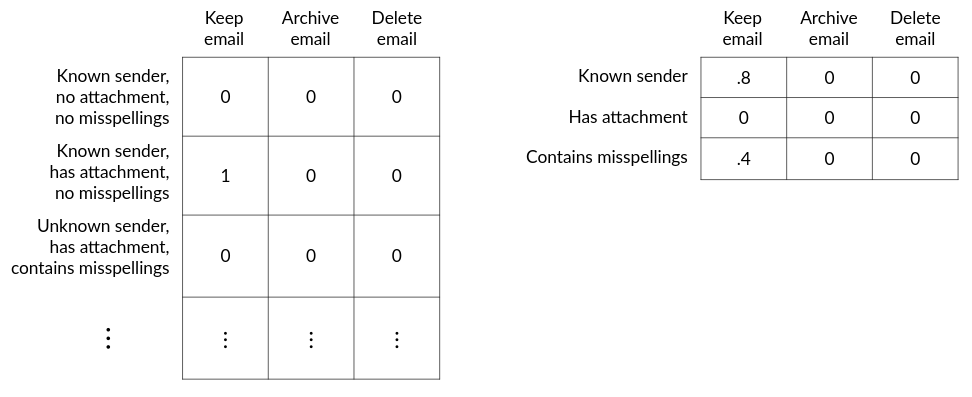
\includegraphics[width=0.9\textwidth]{images/feature_action_array.png}}
\caption{A one-hot state-action array on the left and a FNC feature-action
array on the right for an email routing bot.}
\label{fig:feature_action_array}
\end{center}
\vskip -0.2in
\end{figure*}

In FNC this is a bit different. A feature-action pair is still represented
as a two-dimensional array, but with each row representing a single
feature, rather than a distinct feature array. This gives the tremendous
benefit that the number of rows will stay at a manageable size,
rather than try to encompass every conceivable combination of valid
feature values. (Thank you Naive Bayes!)

This also means that the 2D array will no longer be one-hot.
Many individual feature values may be non-zero at any given moment,
so the corresponding number of feature-action cells will also be non-zero.
The right panel of Figure~\ref{fig:feature_action_array} shows
and example of how this might play out.

Since features can take on any value between zero and one, this also
means that feature-action values will not be limited to one and zero.
It opens up the notion of a feature-action activity, which FNC defines
to be the product of the feature activity and the action activity
(which has already been limited to zero and one).
\begin{equation}
(s_i, a_j) = s_i a_j
\end{equation}

\subsection*{Quirk 5: The condensed trace}
\label{algofeatureactiontrace}

It's common in tabular RL algorithms to track a historical trace of recently
active state-action pairs in order to appropriately attribute reward when it is
encountered. When a reward is finally encountered it gets attributed most
strongly to the most recent state-action pair, with a decay as it reaches
further back in time. For instance, it may use a decay schedule of
attributing the full reward $r$ to $(s_i, a_j)_t$, a discounted reward
$\gamma_r r$ to $(s_i, a_j)_{t-1}$, where $\gamma_r$ is a discount factor
between 0 and 1. From there, an additional factor of $\gamma_r$ is applied at
each time step: $\gamma_r^2$ to the feature-action pair at time $t-2$,
$\gamma_r^3$ at $t-3$, and so on with $\gamma_r^n$ at time $t-n$.

\begin{tabular}{r l}
    reward & feature-state pair\\
    $r$ & $(s_i, a_j)_t$\\ 
    $r \gamma_r$ & $(s_i, a_j)_{t-1}$\\ 
    $r \gamma_r^2$ & $(s_i, a_j)_{t-2}$\\ 
    \vdots & \vdots \\
    $r \gamma_r^n$ & $(s_i, a_j)_{t-n}$\\ 
    \vdots & \vdots \\
\end{tabular}

With a little rearrangent, it is possible to shift the decay from the
reward to the feature-action activities. This is straightforward,
since FNC is already representing the pairs with real values between zero
and one.

\begin{tabular}{r l}
    reward & feature-state pair\\
    $r$ & $(s_i, a_j)_t$\\ 
    $r$ & $\gamma_r (s_i, a_j)_{t-1}$\\ 
    $r$ & $\gamma_r^2 (s_i, a_j)_{t-2}$\\ 
    \vdots & \vdots \\
    $r$ & $\gamma_r^n (s_i, a_j)_{t-n}$\\ 
    \vdots & \vdots \\
\end{tabular}

In this formulation, the decay is applied to the feature-action activities,
rather than to the reward. One way to calulate this is to
reach back in time and incrementally
decay every feature-action pair by an additional factor of $\gamma_r$.

Since FNC is making use of a 2D array to represent
feature-action activites, it can cut a small corner and put the
entire feature-action history of the agent in one array. The the discounting
update at each timestep is a straightforward matter of multiplying
every element in the array by $\gamma_r$.

Using one array to represent the whole history of feature-action activities
means that it will have to account for collisions---times when the same
element in the array has a nonzero value associated with multiple time steps.
The way that FNC resolves this is with the maximum operator. Whichever
of the two values is greater wins.

Putting it all together, 
\begin{eqnarray*}
(\overline{s_i, a_j})_t = \max(&&(s_i, a_j)_t , \\
&&\gamma_r (s_i, a_j)_{t-1},\\
&&\gamma_r^2 (s_i, a_j)_{t-2},\\
&&\cdots,\\
&&\gamma_r^n (s_i, a_j)_{t-n},\\
&&\cdots)\\
\end{eqnarray*}

where $(\overline{s_i, a_j})_t$ is the condensed, discounted history
of the agent's feature-action activities. With a little fancy footwork,
this can become an incremental update, well suited to the iterative computation
that happens in a RL agent.
\begin{equation}
(\overline{(s_i, a_j})_t = \max(
(s_i, a_j)_t , 
\gamma_r (\overline{s_i, a_j})_{t-1})
\end{equation}

The choice of $\gamma_r$ determines how rapidly history is forgotten and
how far back in time an agent's successes and failures can be attributed to its
decisions. An agent playing tic-tac-toe can get by with a $\gamma_r$
of around .7 because it only needs to reach back 4 of 5 moves to cover the
whole game.
An agent solving a maze that takes about 100 moves to solve will
probably want a $\gamma_r$ in the neighborhood of .98 so that it can apply
its learning far enough back in time to be useful on its next pass through
the maze.
And an agent learning to classify a string of unrelated
objects might be best served by a $\gamma_r$ of zero. It would be a mistake
to apply any of the reward to the agent's prior decisions.
Each time step is independent of the last and however it goes, shouldn't
affect the agent's perception of its performance on prior objects.

\subsection*{Quirk 6: Condensed feature history}
\label{algofeaturetrace}

The feature-action trace enables two similar but distinct things.
The first is learning multi-step tasks, as illustrated in the examples above.
The second is compensating for a slow world. If an agent can sense and act very
quickly compared to its world's dynamics, it may take several time steps
before it realizes the reward from an action. A fast agent may throw a
basketball toward a hoop, then perform several iterations through its
RL loop before the ball goes through, earns a point, and earns a reward for the
agent. A condensed history allows the critical feature-action pair from
several moments prior to get its fair share of reward allocated to it.
Alternatively, any time a reward is manually administered by a human
it will be subject to humans' cognitive processing times. Even under the
best of circumstances, this will not be faster than 150 ms. Typically it will
be ten times greater. It's easy for a very chill agent to complete
several iterations in this time.

This trick of accounting for fast/slow system mismatches by spreading
credit across the history of the fast system can be applied to
feature activities on their own too. In an ideal RL system, the sensed
state at each time step would be current and complete (observable),
but in practice it can be both indirect and delayed (partially observable),
as detailed in Quirk No.3 above. When creating feature-action pairs,
this means that it may actually be a feature sensed several time steps
prior that is most relevant to the current action selection.

A natural way for this to manifest is, once a feature is detected,
the underlying state that triggered it remains valid for some time.
For instance, consider a robot that is learning to respond to human
verbal commands. When the human says ``stop", that is sensed by
the robot and reported in the feature array at time step $t$.
However, the underlying state of the system includes the intent of
the human, which may remain for many time steps thereafter until
the robot stops doing whatever it is doing.
Having a condensed representation of feature history gives the robot
a short-term memory for recent features, and allows it a small time
window for experimentation to find the action to pair with the feature
to get a reward.

To allow these connections to be learned, FNC also maintains a
condensed representation of feature history in the same way it
keeps a feature-action history.

\begin{equation}
\overline{s}_{i, t} = \max(s_{i, t}, \gamma_f \overline{s}_{i, t-1})
\end{equation}

where $\gamma_f$ is another discount factor specific to the feature
history. It can have a different value than $\gamma_r$, allowing
for different decay dynamics for the feature history.

In FNC the condensed feature-action trace uses the condensed feature
history instead, so its full expression is
\begin{equation}
(\overline{\overline{s_i}, a_j})_t = \max(
(\overline{s_i}, a_j)_t , 
\gamma_r (\overline{\overline{s_i}, a_j})_{t-1})
\end{equation}

\subsection*{Quirk 7: The do-nothing action}
\label{algodonothing}

The ``do-nothing" action is a special actions included in every FNC model.
It lets the model represent what happens if it deliberately refrains
from taking any actions. If an agent is already in a high reward state and
expects to keep receiving that reward, then its best option is to not
take any new actions, just sit and let the reward
continue to roll in. This could be a robot vacuum sitting on its
charging station, or an interplanetary probe waiting for its next
instruction from earth. In some situations, the best result comes when
the agent nearly sits on its ass and does nothing. The do-nothing action
gives it that option.

\subsection*{Quirk 8: The average action}
\label{algoavgaction}

The second special action in every FNC model is the ``average" action.
It represents what is likely to happen in a given circumstance,
if the model is deliberately blind to which action was taken.
It is a way for the agent to learn when its actions
don’t matter. There are many circumstances where the world is going to do
what the world is going to do and there’s nothing the agent can do
in that moment to change its course. If an agent is watching the clock,
no action that it can take will prevent time from advancing from one
second to the next. An agent that is observing a ball sail through
the air will not be able to alter the ball's course, no matter what it does
(unless perhaps it is a robot with very long arms, or is very good at
throwing rocks). The average action finds the average outcome for
an initial set of features, regardless of the action taken.
It helps the agent to learn what
patterns depend only on the previous state, and not on any action
that was taken. Learning this is useful because it frees the agent up
to make decisions based on other costs and benefits that are causal.

The average action highlights a common assumption of RL agents, namely
that every action they take impinges on the external world in some way.
In adversarial environments, they can spend a lot of resources trying
to learn to influence things that they have no control over. FNC
won’t have any better luck at controlling those things, but it will
at least be able to learn to stop worrying about them.

Here is the full representation of actions generated by FNC 
\begin{equation}
\mathcal{A} = [a_0, a_1, a_2, \cdots, a_j, \cdots, a_m]
\mbox{ where } a_j \in \{0, 1\} 
\end{equation}
Actions are discrete, on or off. Internally to FNC, and in the predictions
it provides to the planner, the do-nothing and average actions are appended
to the array as $a_{m+1}$ and $a_{m+2}$ respectively.

\subsection*{Not a quirk: Reward estimation}
\label{algorewards}

The way reward is learned is anything but quirky. It's more of a classic.
It is the same approach described in
Equation 2.5 of \href{http://incompleteideas.net/book/RLbook2020.pdf}{Sutton and Barto}
in the context of multi-armed bandits, a simple RL scenario.
For a given feature-action pair
\begin{equation}
Q_t = Q_{t-1} + \alpha(r_t - Q_{t-1})
\end{equation}
where is $Q_t$ is the expected value of reward for that
feature-action pair as of time $t$, $r_t$ is the observed value,
and $\alpha$ is a constant learning rate between zero and one,
usually much closer to zero than one.

This is a recursive filter, using the previous time step's value to
estimate the next. It results in a exponentially-weighted moving average
of the reward. The entire history of observed rewards contribute to the
estimate, but recent observations are weighted much more heavily than older ones.
It has the useful properties that it doesn't jump around too much from one
time step to the next (as long as $\alpha$ isn't too large), but it will
converge on the true average value of $r$ (if the average value of $r$
is constant) and will adapt
to any changes in $r$ as well (if its average isn't constant).

The expression above for updating $Q$ only applies when the feature-action
pair $ij$ is active, that is, when feature $i$ has occurred and action $j$ has been
taken. In traditional tabular RL, this is an all-or-nothing proposition, but
in FNC it can by fractionally valued.
Here is the more complete
and explicit version that includes the condensed feature-action history.
\begin{equation}
Q_{ij, t} = Q_{ij, t-1} + \alpha
(\overline{\overline{s_i}, a_j})_t
(r_t - Q_{ij, t-1})
\end{equation}

\subsection*{Quirk 9: Reward prediction}
\label{algoreward prediction}

The recursive reward estimation method above creates a two-dimensional array
of reward estimates where every row represents a feature and every column
an action. In this form it becomes a very helpful source of information
about what actions the agent should take on the following time step.
If it were a traditional tabular learning algorithm, the planning procedure would
be to isolate the row associated with the most recent state observation.
This row would show, for all the possible actions the agent might take,
what the expected reward would be. A greedy agent would pick the action
associated with the highest reward and be done with it. A more exploratory
agent might choose one of the other actions just to learn more about them.
But either way, the action-reward relationship is the foundation on which
these decisions are based.

In FNC many individual features can be active at once, and can be active
at any value between zero and one. There is not just one row of reward
estimates to be pulled out of the array, there are several. The way 
FNC handles this is to do a weighted average of all the rows, based on
their corresponding feature activities. This ensures that rows associated
with highly active features are counted strongly, and rows without 
any significant activity are ignored. $Q_j$ is the predicted reward for
action $a_j$.

\begin{equation}
Q_{j} = \frac{\sum_i Q_{ij} \overline{s_i}}
{\sum_i \overline{s_i}}
\end{equation}

The act of combining reward across features is an important one.
There are many reasonable ways to do it, each with a different outcome.
The choice of a weighted average is a deliberate design decision.
It would also be possible to take the maximum, the sum, the unweighted
average, or to select one of the rewards at random.
Since features are assumed to independent, one way to view the
feature-action reward estaimtes is as an ensemble model, a collection
of simple (and simplistic) models that all cast their votes. How those
votes are tallied from an ensemble is a bit of art. In practice, the
weighted average ended up making the most sense here because it does a good
job of only considering rewards associated with active features, and considering
those rewards with the most active features most heavily.

\subsection*{Quirk 10: Intermittent rewards}
\label{algointermittentrewards}

Intermittent rewards were described in some detail in
Section~\ref{subsec:introintermittent}. FNC allows for rewards to be intermittent,
that is, to be absent on any number of time steps. When there is no reward
to be reported. FNC just skips the reward update on that time step. 
The exponentially decayed moving average doesn't incorporate a new value,
not even a zero, and it doesn't change the estimate for $r$.

\subsection*{Quirk 11: Multiple rewards}
\label{algomultiplerewards}

It’s natural to build a system where both internal and external rewards are at play.
There may even be multiple sources of external reward. When any of these
can be intermittent, this leads to a scenario
where some aspects of the reward signal need to be updated on a given time step
where others do not.

A really bizzare thing that FNC does is that it allows for multiple reward channels. 
(As far as I know it is unique in this respect.)
This allows it to accommodate any number of reward sources, any one of which
may be absent at any given time step.

\begin{equation}
\mathcal{R} = [r_0, r_1, r_2, \cdots, r_k, \cdots, r_l]
\mbox{ where } r_k \in \{\mathbb{R}, \emptyset\}
\end{equation}

FNC handles this by keeping track of $l$ different feature-action reward 
estimates, and only updating estimates on each time step for which it
has a non-null reward.
\begin{equation}
Q_{ijk, t} = Q_{ijk, t-1} + \alpha
(\overline{\overline{s_i}, a_j})_t
(r_{k,t} - Q_{ijk, t-1})
\end{equation}
When it comes time to predict the reward associated
with each action for the next time step, it makes a prediction for each
reward channel individually, with a weighted average as in the method above,
and then it sums the predicted reward across all reward sources.
\begin{equation}
Q_{j} = \sum_k \left ( \frac{\sum_i Q_{ijk} \overline{s_i}}
{\sum_i \overline{s_i}} \right )
\end{equation}

\subsection*{Not so quirky: Transition probability estimation}
\label{algotransitions}

FNC's transition probability calculations are fairly vanilla. 
The only quirks it has are spillovers from its other quirks.
In Markov decision processes, transition probabilities 
to an outcome $s^\prime$ are typically defined
in terms of the most recent state and action.
\begin{equation}
p(s^\prime | s, a)
\end{equation}

The probability is based on the crusty old frequentist technique of
counting all the times the transition happened and dividing it by
all the times it had the opportunity to happen. Considering
specfically the transition from feature $s_i$ to outcome $s^\prime_k$
via action $a_j$.
\begin{equation}
p(s^\prime_k | (s_i, a_j) = \frac
{\mbox{count}(s_i, a_j, s^\prime_k)_t}
{\mbox{count}(s_i, a_j)_t}
\end{equation}

Due to the fact that feature-action pairs and outcomes can have fractional
values, FNC needs to modify this from using $\mbox{count}()$ and use
a sum instead. Also, to ensure that the fraction is well behaved, one is added
to the denominator. This results in a somewhat lower probability estimate
early in FNC's experience, but its influence fades as the number of occurrences
grows.
\begin{equation}
p(s^\prime_k | (s_i, a_j) = \frac
{\sum_t(s_i, a_j, s^\prime_k)_t}
{\sum_t(s_i, a_j)_t + 1}
\end{equation}

In FNC, transition probabilities are defined in terms of the condensed
feature-action activity trace.
\begin{equation}
p(s^\prime | (\overline{\overline{s}, a}))
\end{equation}
And the transition activity is given by the product of the activity trace
and the outcome activity.
\begin{equation}
(\overline{\overline{s_i}, a_j}, s^\prime_k) = 
(\overline{\overline{s_i}, a_j}) s^\prime_{k} 
\end{equation}

All together, this gives FNC's version of transition probabilities.
\begin{equation}
p(s^\prime_k | (\overline{\overline{s_i}, a_j}) = \frac
{\sum_t (\overline{\overline{s_i}, a_j}, s^\prime_k)_t}
{\sum_t (\overline{\overline{s_i}, a_j})_t + 1}
\end{equation}

Although the form of this is very similar to canonical frequentist
probability estimates, FNC's idiosyncracies lead to a slightly different
interpretation. Imagine that feature $s_i$ is fully active when action $a_j$
is taken at time $t$, so that the trace $(\overline{s_i}, a_j)_t = 1$.
Thanks to the trace decay schedule induced by $\gamma_r$ it will
trail off over time, even if no other actions are taken.
The value of the trace at $t + \tau$ will be $\gamma_r^{\tau}$. 

\begin{figure}[ht]
\vskip 0.2in
\begin{center}
\centerline{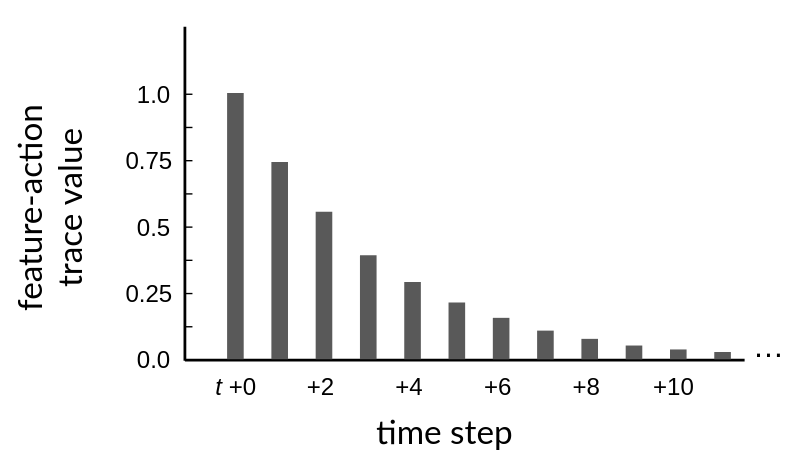
\includegraphics[width=3.0in]{images/trace_decay.png}}
\label{fig:trace}
\end{center}
\vskip -0.2in
\end{figure}

The sum of the trace over time will be the total of all the decayed components.
\begin{equation}
\sum_t (\overline{\overline{s_i}, a_j})_t = (\overline{s_i}, a_j)
\left (1 + \gamma_r + \gamma_r^2 + \gamma_r^3 + \cdots \right )
\end{equation}

This form has its own name,
\href{https://en.wikipedia.org/wiki/Geometric_series#Formula}{geometric series},
and even better, it has a closed form solution.
\begin{equation}
1 + \gamma_r + \gamma_r^2 + \gamma_r^3 + \cdots = \frac{1}{1 - \gamma_r}
\end{equation}

The result of this is that even for a feature-action pair that is active
on a single timestep, a single occurence, the resulting sum of the trace will not
be 1, but will be $1 / (1 - \gamma_r)$. The way this impacts the frequency
calculation is that it inflates the count of the feature-action pair occurrence.
If the outcome $s_k$ occurs with an activity of 1 at time $t$, but is zero
thereafter, then the transition
$(\overline{\overline{s_i}, a_j}, s^\prime_k)$ will only be incremented by 1,
even though the feature-action pair will be incremented by
$1 / (1 - \gamma_r)$. So even if the outcome occurred for a single timestep
every time the feature-action pair of $s_i$ and $a_j$ occurred, it would
still show up with a transition probability of (possibly much) less than one.

The only way that the sum of transition occurrences can keep pace with the
sum of the feture-action occurrences is if the outcome $s_k$ becomes fully active
\textit{and stays active}, at least until the feature-action trace has decayed
to almost nothing. In that case the calculated transition probability will
stay close to one.

All of this gives the method for predicting individual transition probabilities.
It still treats every feature as independent. When in operation, each time step
will bring FNC a new combination of features, each with its own activity level.
It has to aggregate these in come way to come up with an overall conditional
probability estimate $p(s^\prime_k | a_j)$.

FNC does this by multiplying each feature-action-outcome transition probability
estimate by the condensed activity history $\overline{s_i}$ of its
corresponding feature.

\begin{equation}
p(s^\prime_k | a_j) = \max_i (\overline{s_i} \mbox{ }
p(s^\prime_k | (\overline{\overline{s_i}, a_j}))
\end{equation}

This allows FNC to generate a set of what if scenarios for each action.
If a given action is taken, it tells the expected probability of each
outcome feature. The $\max()$ operator works as an aggregator for this, because
it doesn't get weighed down by all the features that aren't currently active
or aren't particularly predictive of a given outcome. All it needs is one
feature-action pair to be confident of a particular outcome for it to embrace it.

\subsection*{Quirk 12: Uncertainty}
\label{algouncertainty}
The last unusual thing that FNC does is to provide an uncertainty estimate
on the transition probabilities. This estimate is approximate, but it
gives a planner some basis for interpreting the transition probability estimates.

Imagine that the outcome FNC is trying to predict is the result of a coin
flip where the coin might be unfair. After two flips, the coin has come up
heads twice. Because it is two for two, FNC will predict that the next flip will
be heads with a probability of one. The entirety of its (extremely limited)
experience leads it to believe this. Of course, we know that even a fair coin
will have its first two flips be the same half of the time. A more honest
estimate should reflect the fact that after two flips we still don’t know
very much.

However, if after 1000 flips the coin has come up heads 900 times, it is
reasonable to predict that it will come up heads nine times out of ten on average,
and to be quite confident in that prediction. It may not be exactly right,
but it’s probably close.

The pattern here is that with more observations uncertainty decreases.
Leaning on statistics helps make this more concrete. In the case of a
biased coin where the outcome is always one of two values, it's natural to
model the outcome using a Bernoulli probability distribution. In the more
general case where an outcome feature can take on any value between
zero and one, a beta distribution is a better fit. It’s very flexible and
can degenerate into a Bernoulli distribution, a uniform distribution,
and a rich set of other shapes, all supported on the interval $[0, 1]$.

The good news for us is that we don’t have to care about any of that.
The \href{https://en.wikipedia.org/wiki/Central_limit_theorem}
{central limit theorem} lets us sidestep it. As long as we can assume that
the outcome is (more or less) independent from one time to the next and
distributed in (pretty much) the same way each time, the central limit
theorem tells us that the mean of a sample will follow a normal distribution,
and that the distribution will have a standard error of
$\sigma^2 / \sqrt{n}$, where $\sigma^2$ is the variance of the sample and
$n$ is the number of observations in it. For a distribution supported on 
$[0, 1]$, $\sigma$ can ever be more than .5. The range
associated with a $95\%$ confidence interval is $\pm 1.96 \sigma / \sqrt{n}$
implying that $\pm 1 / \sqrt{n}$ is a slightly conservative bound for the mean,
a cautious estimate for the uncertainty in FNC's predictions. The the case of
FNC, $n$ is the number of times a feature action pair has occurred.
(Note that, as was just called out in the previous section, FNC overcounts
this by $1 / (1 - \gamma)$ due to how it handles trace decay.

Another shortcut that FNC takes is reporting $1 / n$ instead of $1 / \sqrt{n}$.
This is pure laziness, just to save FNC some computation.
It results in an uncertainty
estimate that smaller, reflecting a somewhat lower confidence level.
Also, since 
the number of occurrences of a feature-action pair can be arbitrarily small,
$1/n$ can be arbitrarily big. To keep it properly limited to be no greater than
one, an extra observation is added to $n$. The actual uncertainty estimate FNC
returns after all these modifications, $\delta$, is given by
\begin{equation}
\delta_{ij} = \frac{1}{1 + \sum_t(\overline{\overline{s_i}, a_j})}
\end{equation}

A planner that consumes the uncertainty has the option fix the uncertainty
estimates, to subtract the extra observation, to take the square root
and to apply a $1 / (1 - \gamma_r)$  correction
to get a more accurate confidence interval. Or it can also just accept $1 / (1 + n)$
as a rough approximation built on a scaffold of assumptions,
some generous, some conservative.

As with the transition probabilities, it is also necessary to aggregate the
conditional uncertainties, the uncertainties across
all the currently active features.
And as with the transition probabilities, the $\max()$ operator is the 
aggregator of choice. Specifically the uncertainty associated with a given
action $\delta_j$ is the maximum of all the features-action uncertainties
$\delta_{ij}$, each multiplied
by the recent feature activity history $\overline{s_i}$.

\begin{equation}
\delta_j = \max_i (\overline{s_i} \mbox{ } \delta_{ij})
\end{equation}

There are several other defensible ways to aggregate uncertainties,
but the choice of the maximum is deliberate. It ensures that whichever
aspect of the current situation is the most uncertain,
whichever feature has been paired
with this action the fewest times, gets to dominate.
